\documentclass[a4paper,12pt]{article}

\usepackage[pdftex]{graphicx}
\usepackage{amsmath,amsfonts,amsthm}
\usepackage{fullpage}

\newtheorem{lemma}{Lemma}

\newcommand{\floor}[1]{\ensuremath{\left\lfloor #1 \right\rfloor}}

\author{April Camp 2017}
\title{Test 2 -- Solutions}
\date{}

\begin{document} \maketitle

\begin{enumerate}
	\item 
	\textit{For an integer $N>0$, $N$ boys, no two of them having the same height, are arranged in a circle. A boy in the given arrangement is said to be \emph{tall} if he is taller than both of his neighbours; a boy is said to be \emph{short} if he is shorter than both of his neighbours. Prove that the number of tall boys in the circle is equal to the number of short boys in the circle.}
	
    Consider any arbitrary arrangement of the boys along the circle. We put the
    signs ``+" or ``-" before each boy in accordance with the following rule:
    we move clockwise along the circle, and put the sign ``+" before the boy if
    he is taller than the previous boy, and we put the sign ``-" if he is
    shorter than the previous one.

    It is evident that a boy is tall if and only if the sign ``+" stands before
    him, and the sign ``-" stands after him. Similarly, a boy is short if and
    only if the sign ``-" stands before him, and the sign ``+" stands after
    him. (Note that the tallest of the $N$ boys is tall, so both the signs
    ``+" and ``-" exist in every configuration.)

    Therefore the number of tall boys in the arrangement is equal to the number
    of alternations of ``+" and ``-", and the number of short boys is equal
    to the number of alternations of ``-" and ``+". Regarding all
    successive ``+" signs as a single ``+" sign, and all successive ``-" signs
    as a single ``-" sign, we construct a new arrangement of signs. It is easy
    to see that the number of alternations of ``+" and ``-" in the initial
    arrangement is equal to the number of alternations of ``+" and ``-" in the
    new arrangments, and similarly for the number of alternations of ``-" and
    ``+". But it is evident that the number of alternations of ``+" and ``-" in
    the new arrangement is equal to the number of alternations of ``-" and
    ``+", and so the numbers of tall boys and of short boys in the
    arrangement are equal.
	
		
	\item 
	\textit{Nonzero real numbers $a,b,c,d$ satisfy the equations \[a+b+c+d = 0, \qquad \frac{1}{a}+\frac{1}{b}+\frac{1}{c}+\frac{1}{d}+\frac{1}{abcd} = 0.\]
	Find all possible values of the product $(ab-cd)(c+d)$.}
	
	Clearing denominators in equation two, we get $abc +bcd +cda +dab = -1$. Hence \begin{align*} (ab-cd)(c+d) &= abc +abd -cd(c+d) \\ &= -bcd -cda -1 -cd(c+d) \\ &= -1 -cd(a+b+c+d) = -1.\end{align*}
	
	\item
	\textit{Find all primes $p$ such that $5^p +4p^4$ is the square of an integer.}
	
Suppose that $5^p + 4p^2 = k^2$. Then we have that
\[
	(k - 2p^2)(k + 2p^2) = 5^p,
\]
and so both $(k - 2p^2)$ and $(k + 2p^2)$ are powers of $5$. Let
\begin{align*}
	k - 2p^2 & = 5^a & & \text{and} & k + 2p^2 & = 5^b.
\end{align*}

Then we have that
\[
	4p^2 = 5^b - 5^a.
\]

We clearly have that $5^b > 5^a$, and so this expression is divisible by $5^a$.
If $a > 0$, then we see that $4p^2$ is divisible by $5$, and hence $p=5$.
We have that
\[
	5^5 + 4\cdot 5^4 = 5^4 (5 + 4) = (5^2 \cdot 3)^2,
\]
and so $p=5$ is a solution.

We now consider the case where $a=0$. In this case, we have that $b=p$, and so
we find that
\[
	5^p = 4p^2 + 1.
\]

However, one can prove by induction that
\[
	5^n > 4n^2 + 1
\]
for all $n > 1$, and so we have no solutions in this case.
	
	\item 
	\textit{$ABCD$ is a cyclic quadrilateral. Let the circle $\Gamma_1$ pass through $A$ and $B$ and touch $CD$ at $E$; let the circle $\Gamma_2$ pass through $B$ and $C$ and touch $DA$ at $F$; let the circle $\Gamma_3$ pass through $C$ and $D$ and touch $AB$ at $G$; and let the circle $\Gamma_4$ pass through $D$ and $A$ and touch $BC$ at $H$. Prove that $EG \perp FH$.}
	
    {\centering 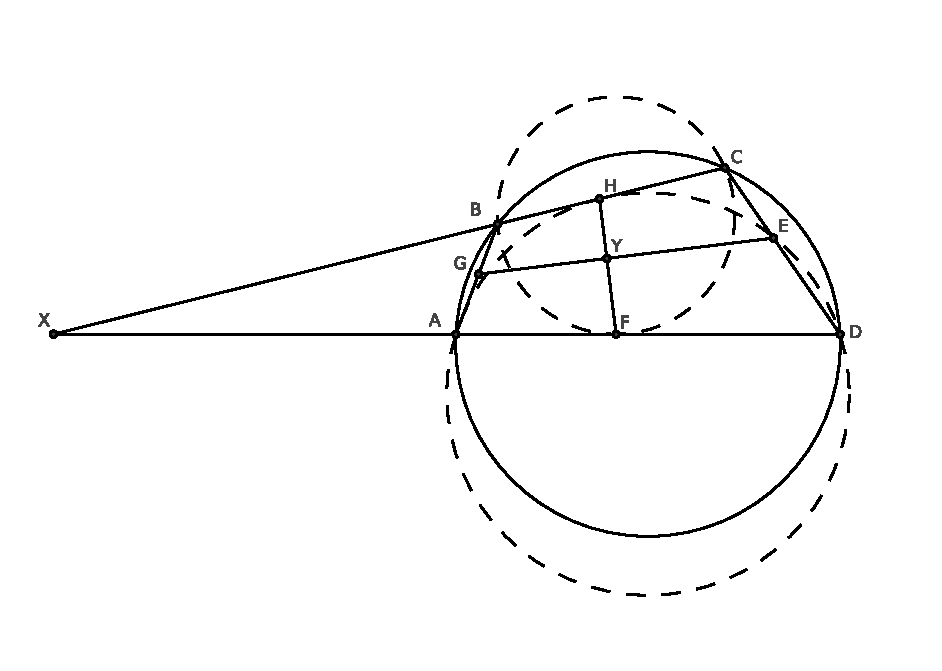
\includegraphics[width=0.9\textwidth]{T2Q4.eps} }
    
    If the quadrilateral $ABCD$ has a pair of parallel sides, the result follows
    from the symmetry of the construction. So we suppose that $ABCD$ is not a
    trapezoid or a rectangle.

    Let $X = BC \cap AD$. Since $\Gamma_2$ touches $AD$ at point $F$, we have
    that $XF^2 = XB \cdot XC$.

    Similarly, $XH^2 = XA \cdot XD$. Since $ABCD$ is cyclic, we have that
    $XB \cdot XC = XA \cdot XD$, and so $XF = XH$, and hence $\triangle XHF$ is
    an isosceles triangle. Thus $\angle BHF = \frac{1}{2} (180^\circ - \angle
    CXD) = \frac{1}{2}(\angle C + \angle D)$.

    Similarly, $\angle BGE = \frac{1}{2} (\angle A + \angle D)$.

    Let $GE \cap HF = Y$. Then $\angle GYH = 360^\circ - \left(\angle B +
        \frac{1}{2} (\angle C + \angle D) + \frac{1}{2} (\angle A + \angle
        D)\right) = 360^\circ - (\angle B + \angle D) - \frac{1}{2} (\angle A +
    \angle C)$.

    Since $\angle A + \angle C = \angle B + \angle D = 180^\circ$, we have
    $\angle GYH = 360^\circ - 180^\circ - 90^\circ = 90^\circ$, and so $EG
    \perp FH$.
	
	\item
	\textit{Given a polynomial $P$ with positive real coefficients, show that $P(1)P(xy) \geq P(x)P(y)$ for all $x,y \geq 1$.}
	
	Let the polynomial $P$ be $P(t) = a_n t^n +a_{n-1} t^{n-1} +\dotsb +a_1 t +a_0$ where the $a_i$ are positive.
	
	\textbf{Solution 1:} Note that the sequences $(x^n, x^{n-1}, \dotsc, x, 1)$ and $(y^n, y^{n-1}, \dotsc, y, 1)$ are both decreasing. Hence by the weighted version of Chebyshev's Inequality with weights $w_i = a_i/(a_n+a_{n-1}+\dotsb+a_1+a_0)$,
	\begin{align*}
		&\mspace{24mu} \frac{a_n x^ny^n +a_{n-1}x^{n-1}y^{n-1} +\dotsb +a_1 xy +a_0}{a_n+a_{n-1} +\dotsb +a_1 +a_0} \\ &\geq \frac{a_n x^n +a_{n-1}x^{n-1} +\dotsb +a_1 x +a_0}{a_n+a_{n-1} +\dotsb +a_1 +a_0} \frac{a_n y^n +a_{n-1}y^{n-1} +\dotsb +a_1 y +a_0}{a_n+a_{n-1} +\dotsb +a_1 +a_0} \\
		\mspace{-36mu} \iff P(1)P(xy) &= \left(a_n +\dotsb +a_1 +a_0\right) \left(a_n(xy)^n +\dotsb +a_1 xy +a_0\right) \\ &\geq \left(a_nx^n +\dotsb +a_1 x +a_0\right) \left(a_ny^n +\dotsb +a_1 y +a_0\right) \\ &= P(x)P(y)
	\end{align*}
	\textbf{Solution 2:} Let $x = e^s$ and $y = e^t$ where $s,t \geq 0$. We use H\"older's Inequality twice with the sequence $P = (a_n e^{n(s+t)}, a_{n-1} e^{(n-1)(s+t)}, \dotsc, a_1 e^{s+t}, a_0)$ and the sequence $A = (a_n, a_{n-1}, \dotsc, a_1, a_0)$. First we use it with exponents $s/(s+t)$ for $P$ and $t/(s+t)$ for $A$, giving \begin{align*} P(xy)^{s/(s+t)} P(1)^{t/(s+t)} &= P\!\left(e^{s+t}\right)^{s/(s+t)} P(1)^{t/(s+t)} \\ &= \left(a_n e^{n(s+t)} +\dotsc +a_0\right)^{s/(s+t)} \left(a_n +\dotsc +a_0\right)^{t/(s+t)} \\ &\geq a_n e^{ns} +\dotsc +a_0 = P(e^s) = P(x)\end{align*} and then with exponents $t/(s+t)$ for $P$ and $s/(s+t)$ for $A$, giving \begin{align*} P(xy)^{t/(s+t)} P(1)^{s/(s+t)} &= P\!\left(e^{s+t}\right)^{t/(s+t)} P(1)^{s/(s+t)} \\ &= \left(a_n e^{n(s+t)} +\dotsc +a_0\right)^{t/(s+t)} \left(a_n +\dotsc +a_0\right)^{s/(s+t)} \\ &\geq a_n e^{nt} +\dotsc +a_0 = P(e^t) = P(y).\end{align*}
	Multiplying these inequalities of positive numbers together, we get that \[P(xy)P(1) = P(xy)^{s/(s+t)} P(1)^{t/(s+t)} \times P(xy)^{t/(s+t)} P(1)^{s/(s+t)} \geq P(x) P(y),\] as desired.

\end{enumerate}

\end{document}
